\documentclass[a4paper]{article}
\usepackage{tikz}
\usepackage{amsmath, amsthm, amsfonts, amssymb}
\usepackage{braids}
\usepackage{float}
%Define theorem formatting
\newtheorem{lemma}{Lemma}

\begin{document}
A standard notion in the theory of group representations is the group algebra: if $G$ is a group, then $k[G]$ is the set of all formal linear combinations of the form
\[
   \sum_{g \in G}a_g g
\]
where $a_g \in k$, and only finitely many of the $a_g$ are nonzero. This is clearly an additive group, but it is also a ring, since we can extend the multiplication in $G$ to multiplication in $k[G]$ by extending by linearity.

We can say that $k[G]$ is the $k$-algebra generated by elements of $G$ with the multiplication of generators being the multiplication in the group.
A representation of this group is equivalent to a module over $k[G]$.
In particular, $k[G]$ defines a representation (the regular representation) since it is a module over itself.

There are two particularly natural types of representations: those induced by submodules and quotient modules of $k[G]$ as a module over itself. For finite groups all irreducible representations arise in this way.

The goal here is to describe a particular finite dimensional quotient of $k[G]$, where $G$ is the braid group, the Temperley-Lieb algebra. 

\section{A Presentation of the Braid Group}
We'll take for granted the following presentation of the braid group:
\[
    B_n = \langle \sigma_1, \sigma_2, \dots, \sigma_n : \sigma_i \sigma_j = \sigma_j \sigma_i \text{ if }|i-j| > 1, \sigma_i \sigma_{i+1}\sigma_i = \sigma_{i+1} \sigma_i \sigma_{i+1} \rangle
\]

These generators can be thought of as twists on braids, such as $\sigma_1$ and $\sigma_2$ below:

\begin{center}
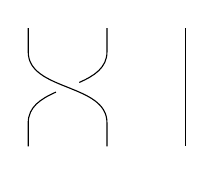
\begin{tikzpicture}
    \braid[number of strands=3] (braid) a_1;
\end{tikzpicture}
\hspace{1in}
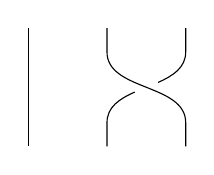
\begin{tikzpicture}
    \braid[number of strands=3] (braid) a_2;
\end{tikzpicture}
\end{center}

Associated to this is a group algebra, $k[B_n]$, which is an infinite dimensional vector space.

\section{The Hecke Algebra}

The symmetric group has a similar presentation to the braid group:
\[
    S_n = \langle \sigma_1, \sigma_2, \dots, \sigma_n : \sigma_i \sigma_j = \sigma_j \sigma_i \text{ if }|i-j| > 1, \sigma_i \sigma_{i+1}\sigma_i = \sigma_{i+1} \sigma_i \sigma_{i+1}, \sigma_i^2 \rangle
\]
(This is saying that $S_n$ is the Coxeter group associated to $B_n$, which happens to be an Artin-Tits group of spherical type, whatever that means,)

Notice that this implies that the symmetric group is a quotient of the braid group, produced by quotienting out by the relations $\sigma_i^2 = 1$.

The Hecke algebra is sort of an `interpolation' from the braid algebra to the grouop algebra of the symmetric group. It is the quotient of the braid algebra, defined by
\[
    H_n(q) = k[B_n] / (\sigma_i^2 = 1 + (q + q^{-1})\sigma_i)
\]
Technically, in order to do this, we need to adjoint an indeterminant $q$, but people seem to get around this by making $q$ a fixed number, in which case, the Hecke algebra is actually a family of algebras, parameterized by $q$.

Inside the Hecke algebra, there are some special elements, namely, the ones of the form $e_i = q - \sigma_i$. These are special because they are idempotent up to a constant multiple: 
\begin{align*} 
(q-\sigma_i)^2&=q^2 - 2q\sigma_i + \sigma_i^2\\
        &=q^2 - 2q\sigma_i + 1+(q+q^{-1})\sigma_i\\
        &=q^2+1 - (q-q^{-1})\sigma_i\\
        &=(q-q^{-1})(q-\sigma_i)\\
        &=(q-q^{-1})e_i
\end{align*}
Also notice a few things: the $e_i$ also generate the whole Hecke algebra, since the $\sigma_i$ can easily be expressed in terms of the $e_i$.
Also, notice that this idempotence property does not depend on any of the braid relations, and just this added relation in the definition of the Hecke algebra (and indeed, this Hecke algebra construction can be done for a wide range of groups).

An important observation is that the Hecke algebra is finite dimensional as a $k$-vector space; you can see this because the symmetric group algebra is finite dimensional, and there is a map sending $\sigma_i$ in the Hecke algebra to $\sigma_i$ in the symmetric group algebra which is an isomorphism of vector spaces (though not as algebras)!

\section{The Temperley-Lieb Algebra}
The Temperley-Lieb algebra is a further quotient of the Hecke algebra, with an additional relation given by 

\[
    Tl_n(q) = H_n(q) / (e_i e_{i+1} e_i = e_i)
\]


It turns out that there is a nice presentation of the Temperley-Lieb algebra in terms of the $e_i$, namely
\[
    Tl_n(q) = \langle e_1, e_2, \dots, e_n : e_i e_j = e_j e_i \text{ if }|i-j| > 1, e_i e_{i+1}e_i = e_{i+1}, e_i^2 = (q+q^{-1})e_i \rangle
\]

$Tl_n(q)$ is finite dimensional, since the Hecke algebra was finite dimensional. We can give a certain basis of $Tl_n(q)$ in terms of pictures, much like we can with the braid algebra.

These pictures will be of `noncrossing matchings'. A noncrossing matching consists of a square with $n$ marked points on the top, and $n$ marked points on the bottom, where each marked point is connected to another marked point by a path (note that there is no condition that the marked points need to be matched with marked points on the other side of the square).


% <!-- TODO: Draw the diagrams here -->

$TL_n(q)$ is spanned (as a vector space over $k$) by square diagrams, with $n$ distinct endpoints on top, and $n$ distinct endpoints on the bottom, and each endpoint is connected to another endpoint with a strand (which is only defined up to homotopy). There is no constraint that endpoints on the top should be connected to endpoints on the bottom, but there is the constraint that these strands must be noncrossing. 

The multiplication is then produced by concatenating these diagrams, combining them tip to tail, and matching up the endpoints, and also by the relation that any circles that appear in the diagrams are equal to $q$. 

If you're keeping track, the single twist braids that generate the braid group are sent to the element $q - e_i$ in the Temperley-Lieb algebra, which looks like the following picture:

% <!--  Draw picture -->
If we let $q = x^{1/2} - x^{-1/2}$ in this relation, then in fact, this looks a lot like the Skein relations defining the Jones polynomial. (As an aside, in graph theory and matroid theory, there is the notion of a Tutte polynomial, which resembles the Jones polynomial in a lot of ways, and in the same spirit as this, there is an algebra known as Tutte-Grothendieck ring, which encodes properties of a graph which can be defined using `minor' relations).

\section{Dimension of the Temperley-Lieb Algebra}
Take a diagram that looks like 

% <!-- TODO: Draw the diagrams here -->

and imagine slicing this diagram in half (only slicing through paths going from the top to the bottom), and arranging the endpoints on a single line. Then, reconnect the endpoints of the cut paths. This gives a drawing that looks like a bunch of nested mountain ranges, which do not intersect. On the other hand, given such a mountain range, we can also get a Temperley-Lieb diagram by restacking these points.

% <!-- TODO: Draw the diagrams here -->

Given such a set of nested mountain ranges, we can define a set of matching parentheses on the $2n$ points, namely, we put a left parenthesis at the start of each range, and a right parenthesis at the end. This gives a bijection between the Temperley-Lieb diagrams and valid nested parentheses. We can count such nested parentheses using the $n^{th}$ Catalan number, 
\[
C_n = \frac{1}{n+1}\binom{2n}{n}
\]


\section{Irreducible Submodules of the Temperley-Lieb Algebra}
Whenever we have an algebraic structure, it's interesting to try decomposing it into smaller pieces. Ideally, we would go ahead and decompose it into pieces which themselves cannot be decomposed. In particular, when we have an ring, we can think of it as a module over itself and look for a decomposition into simple submodules (modules with no proper submodules other than 0). A ring that has this property is said to be semisimple. The Artin-Wedderburn theorem asserts that if we have an Artinian semisimple ring (in particular, any semisimple algebra over a field), is isomorphic to the product of matrix rings over a division algebra.

Maschke's theorem says that whenever we have a finite group $G$ (and $k$ is a field whose characteristic does not divide the order of the group), then $k[G]$ is a semisimple ring, and we can show something similar for the Temperley-Lieb algebra.

\subsection{ Jones-Wenzl Idempotents}
The first step to getting such a decomposition into irreducible pieces is finding an idempotent. One way to motivate this is that idempotents in a matrix algebra are the same as projections onto a subspace, and these projections will let us pick out the right invariant subspaces.

We want $p \in Tl_n(q)$, so that $p_n^2 = p_n$. In fact, we'll find $p$ satisfying two stronger conditions:

1. $p_n = 1 + X$, where $X$ is in the span of the nonidentity Temperley-Lieb diagrams.
2. $e_ip_n = p_ne_i = 0$ for each generator $e_i$.

\begin{lemma}
    Lemma 1
\end{lemma}
> If $p_n$ satisfies these conditions, then $p_n$ is an idempotent.

\begin{proof}
\[
    p_n^2 = p_n(1+X) = p_n + p_nX
\]
Notice that because $X$ is in a linear combination of nonidentity Temperley-Lieb diagrams (each of which is generated multiplicatively by the $e_i$), we see that $p_nX = 0$.
\end{proof}


Consider now the ideal generated by $p$. We see that this is in fact 1 dimensional, and spanned as a vector space by $p$. 

Now, we need to construct such a $p$. We can even draw the diagram for this thing explicitly using induction:

%<!-- Draw a diagram here -->


\subsection{Trivalent Trees and Other Irreducible Representations}
One way to get other cool elements of the braid algebra is by combining the various $p_n$, by considering them as a black box. For example,

%<!-- TODO: Draw the diagrams here -->

We can do this by thinking of an element $p_n$ as being a black box that takes in as input $n$ strands and outputs $n$ strands.


<!-- TODO: Describe Trivalent graphs -->
If we have 3 such black boxes, we can draw them together in the plane.

<!-- TODO: Draw the diagrams here -->

In general, we can make larger diagrams that look like this locally, which graphically are trivalent trees, and we can represent a particular element of the Temperley-Lieb algebra by labelling the edges of this tree to represent drawing

For any such diagram, there is always a point which is the closest to the leaves on the top, which is a parent of all of the leaves on the top. 



\subsection{Markov Trace}
We can form a special trace operation as follows: given any braid diagram, we can draw an additional strand (going outside the diagram) connecting each endpoint on the top with the corresponding endpoint on the bottom.
This will produce a collection of circles, and by our relations, we know that circles should be equal to $q$.
Extending this by linearity gives us a map from $Tl_n(q)$ to $\mathbb{R}$.

Geometrically, it is clear that this trace satisfies the cyclic property:
\[
tr(AB) = tr(BA)
\]
for any $A, B \in Tl_n(q)$.

%<!-- TODO: Draw the diagrams here -->

\subsection{Quantum Integers (aka $q$-analogues)}

We define a quantum integer to be 
\[
    [n] = \frac{A^{2n} - A^{-2n}}{A^2 - A{-2}} = \sum_{i=0}^{n-1} A^{4i-2n+2}
\]

We have the relation that $[2][n] = [n+1]+[n-1]$.

\begin{lemma}
If $p_n$ satisfies these conditions, then $p_n$ is an idempotent.
\end{lemma}

\begin{proof}
We can prove this by induction.

Notice that because $X$ is in a linear combination of nonidentity Temperley-Lieb diagrams (each of which is generated multiplicatively by the $e_i$), we see that $p_nX = 0$. $\square$
\end{proof}

\subsection{Orthogonality for Trivalent Graphs}
When $A, B$ are diagrams in different parts, then we want to show that
\[
    tr(\bar{A}B) = 0
\]

If we draw this as a diagram, this looks like
%<!-- Draw diagram -->

%Notice that there are some `bubbles' in the center of this diagram. We need to pop them, and get
%%<!-- draw diagram -->
%Now, if we have a picture like below, and $a > a'$, then we can see that there will be a strand going from $a$ back to $a$, and we will get 0. Doing out the computation further, we can get the following:
%     |
%     |
%     | a
%     |
%     |
%    / \                           
%   /   \                   ------ a ------  |
%b  \   / c = \delta_{a,a'} |_____ b _____|  |
%    \ /                    |_____ c _____|  a
%     |                           -          |
%     | a'                       | | a       |
%     |                           -          |
%                                 ^
%                                 |-----------------this is a scalar
%By repeatedly applying this relation, we can reduce the inner product of any two of these labelled trees to a scalar, and we can see that they are 0 if they are not the same.
%## Changing Trees
%Each trivalent tree gives rise to a particular basis for the Temperley-Lieb algebra, and we can transform between them with a change of basis. We can figure out the coefficients of these linear transformations by using the orthogonality property of the inner product.
%
%The coefficents can be computed using some difficult computations, all of which can be expressed in terms of Pochhammer symbols.
%a   b     c                             d    e    f 
%\   /    /                              \    \   /  
% \ /    /                                \    \ /    
%  \    /       = F_{a,b,c}^{d,e,f}        \    /     
%   \  /                                    \  /        
%    |                                        |            
%    
%\       /                           \         /
% \     /                             \       / 
%  \   /                               \     /
%   \ /                                 \   /
%    |         = F_{a,b,c}^{d,e,f}        -    
%   / \                                 /   \
%  /   \                               /     \  
% /     \                             /       \ 
%/       \                           /         \
%    
%    
%##  An algorithm for evaluating 
%Abstractly, a triavalent graph with no leaves is essentially a scalar, so let's induct on the number of faces, if we draw this on the plane, look at 
%
%\       /                           \         /
% \     /                             \       / 
%  \   /                               \     /
%   \ /                                 \   /
%    |   face     = F_{a,b,c}^{d,e,f}     -    face
%   / \                                 /   \
%  /   \                               /     \  
% /     \                             /       \ 
%/       \                           /         \
%Removes one edge of some face. Repeatedly do this until face has only 2 edges, and then we can remove the face.
%## The Jones Representation
%The braid group acts on noncrossing planar matchings using the Kauffman bracket.
%It is possible to change bases amongst the various trivalent graphs.
%
%We have two basis elements for $TL_2(q)$: $p_1 = \sigma_1$ and $p_2 = 1 - \frac{1}{d} \sigma_1$, and the action on of $TL_2(q)$ is diagonal in this basis (since the group is abelian, and these are irreps).
%
%In general, if $V_i$ is some basis element of $Tl_n(q)$ (using the left-most branching rule for our tree), then
%\[
%    \sigma_1 V_i = \begin{cases} -A^{-3} V_i \text{ if top left edge is }0\AV_i \text{ if the top edge is } 2  \end{cases}
%\]
%This can be seen using pictures.
%The order of $\rho(\sigma_1)$ is infinite if $A$ is not a root of unity.
%
%For each generator of $B_n$, we can choose some tree structure on $Tl_n(A)$ so that the generators act diagonally, (in particular, any tree where the $i$ and $i+1$ strands are connected together by a node), i.e. each generator of $B_n$ has eigenvectors which correspond to a tree structure.
%
%In order to prove this, we needed two facts, that we can change basis so that 
%\       /                           \         /
% \     /                             \       / 
%  \   /                               \     /
%   \ /                                 \   /
%    |         = F_{a,b,c}^{d,e,f}        -    
%   / \                                 /   \
%  /   \                               /     \  
% /     \                             /       \ 
%/       \                           /         \
%And that 
%
%
%
%
%  \   /                     |         |
%   \ /                      |         |
%    x                       |         |
%   / \                      |         |
%  /   \                     |         |
% /     \                    |         |
%/       \                   |         |
%\       /                   \         /
% \     /                     \       / 
%  \   /                       \     /
%   \ /                         \   /
%    |         = R^{1,1}_n        |    
%    |                            |    
%    |                            |    
%    |                            |    
%
%This can all be redone in any braided tensor category.
%
%
\end{document}
